\chapter{METHODOLOGY}
The methodology will follow the Figure \ref{fig:Methodology}.

\begin{figure}[h!]
    \centering
    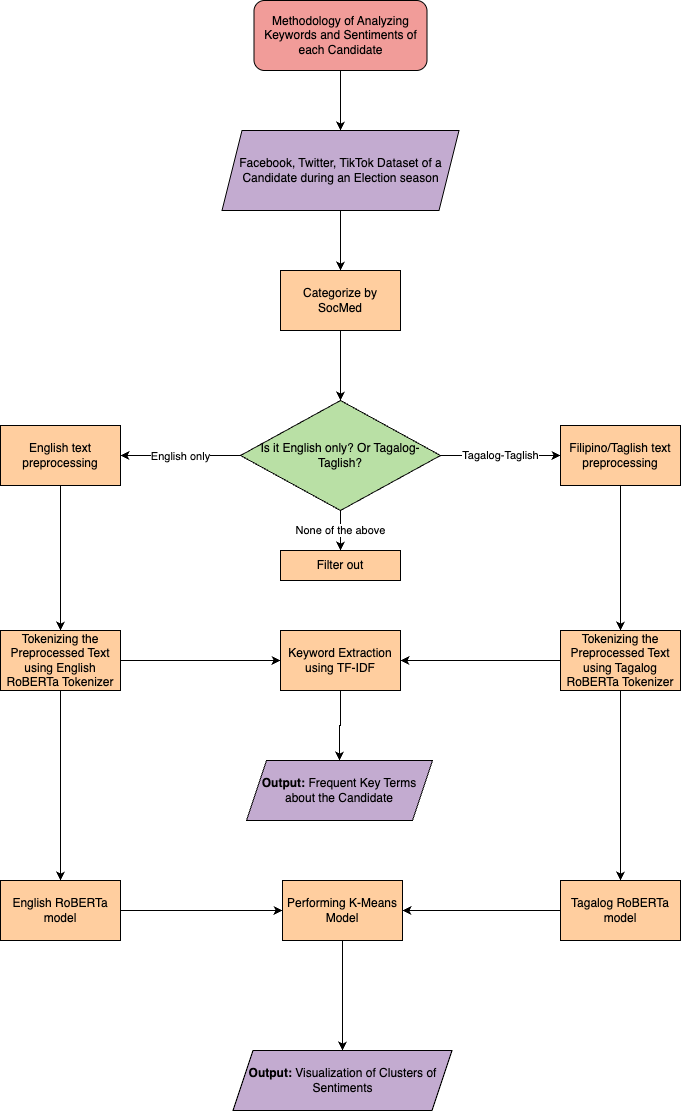
\includegraphics[width=0.82\textwidth]{Figures/methodology_flowchart.png}
    \caption{Methodology Flowchart}
    \label{fig:Methodology}
\end{figure}

\clearpage

\section{Data Collection}
The collection of datasets will happen through the official Application Program Interfaces (APIs) of Twitter, Facebook, and TikTok. If the said APIs are unavailable or country-restricted, open-source tools will be used to collect posts and comments. Due to the unique nature of TikTok, which consists of either images or videos, it will just consist of captions of the video and comments. 

The dates of the posts and comments in the data will be as follows, starting from the day one of the candidates announced their nomination up to two days before the election day. In collecting data based on the given timeframe, there should be at least one of the key terms present:
\newline

\begin{table}[h]
    \centering
    \begin{tabularx}{\textwidth}{X|X|c|c}
        \textbf{Presidential Election years} & \textbf{Intention to Run Announcement} & \textbf{End Date} & \textbf{Key Terms}\\
        \hline\hline
        \multirow{2}{*}{2016} & Duterte and Cayetano: November 21, 2015 & \multirow{2}{*}{May 7, 2016} & \multirow{2}{4cm}{Duterte, Cayetano, Mar Roxas, Roxas, Robredo, Leni, Robredo, DU30, Roro} \\
        & Roxas and Robredo: July 31, 2015 & & \\ 
        \hline
        \multirow{2}{*}{2022}& Marcos and Duterte: October 5, 2021 & \multirow{2}{*}{May 7, 2022} & \multirow{2}{4cm}{Marcos, Duterte, Robredo, Kiko, Pangilinan, BBM, Leni, DU30, Uniteam, Bongbong} \\
        & Robredo and Pangilinan: October 7, 2021 & & \\
    \end{tabularx}
    \caption{Table for Philippine Dataset Ranges}
\end{table}
\begin{table}[h]
    \centering
    \begin{tabularx}{\textwidth}{X|X|c|c}
        \textbf{Presidential Election Year} & \textbf{Intention to Run Announcement} & \textbf{End Date} & \textbf{Key Terms}\\
        \hline\hline
        \multirow{2}{*}{2020} & Biden and Harris: April 25, 2019 & \multirow{2}{*}{November 6, 2020} & \multirow{2}{4cm}{Biden, Harris, Kamala, Trump, Pence, Joe Biden, Donald Trump} \\
        & Trump and Pence: January 21, 2017 & & \\ 
        \hline
        \multirow{2}{*}{2024}& Trump and Vance: November 15, 2022 & \multirow{2}{*}{November 6, 2024} & \multirow{2}{4cm}{Harris, Walz, Trump, Vance, Kamala, JD Vance} \\
        & Harris and Walz: July 21, 2024 & & \\
    \end{tabularx}
    \caption{Table for United States Dataset Ranges}
\end{table}


Each collected post or comment mentioning a candidate(s) will be in the \texttt{.csv} file separately, with each row marked by which social media platform it comes from. They will be utilized separately according to the election year and country for text classification.

\section{Data Preprocessing}
After grouping the datasets, before they are fed into the RoBERTa tokenizer, posts and comments will undergo preprocessing before feeding the data into the RoBERTa model. Since RoBERTa recognizes the stop words such as “the,” “a,” “is”, etc., it will not be removed during this process. The following steps to preprocess the text will be as follows:

\begin{enumerate}
    \item Omitting texts from the dataset if it is not in English, Tagalog, or Taglish.
    \item Removing punctuation marks that have no significance for sentiment analysis.
    \item Replacing emojis with special tags.
    \item Removing unnecessary emojis or replacing emojis with special tags describing them if it is necessary for sentiment analysis.
    \item Lowercasing the text.
    \item Handling links and email addresses by replacing them with a placeholder.
    \item Removing whitespaces and replacing multiple spaces with a single space.
    \item Adding paddings to equalize the length of sentences.
\end{enumerate}

The preprocessed dataset will be placed in a \texttt{.csv} file.

\section{Text Classification and Visualization}
After the preprocessing, the dataset will be fed into the following models: the RoBERTa model for contextualized embedding and the TF-IDF model for determining frequent keywords.

Since the standard RoBERTa model primarily uses an English dataset for pretraining, to handle Tagalog and Taglish language texts, the researchers will use the Tagalog RoBERTa model created by \textsc{DOST ASTI} \cite{MTHD_RoBERTa-model}. The preprocessed dataset will be fed into the RoBERTa Tokenizer before the tokenized result will go into the embedding model. After the formulation of embeddings, they will be fed into the K-Means model so that they will be assigned to the clusters that are essential for creating the visualization of the sentiments based on the semantic similarity of the texts, visualizing the echo chambers. This will be used to compare and contrast the social media presence and activity of each candidate.

Meanwhile, the tokenized texts will also go to the TF-IDF model to determine the frequency of words. The frequency of the words is sorted by how frequently they are used in a certain post or comment. The top 30 keywords per candidate will be used to compare and contrast with other candidates, especially if they are from another country.

\begin{figure}[H]
    \centering
    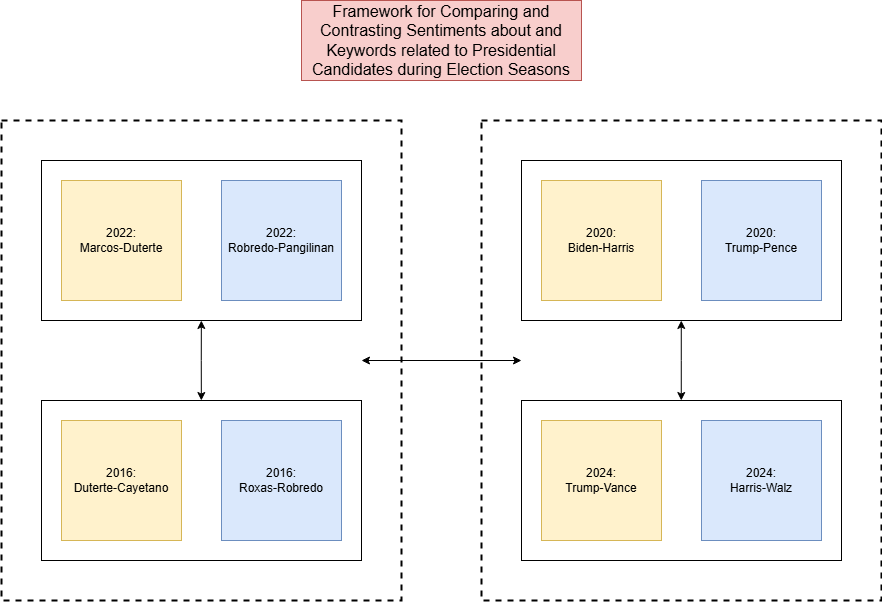
\includegraphics[width=0.82\textwidth]{Figures/methodology_framework-for-comparing.png}
    \caption{Framework for Comparing and Contrasting Sentiments}
    \label{fig:Framework-for-sentiments}
\end{figure}